\documentclass[conference]{config/paper/IEEEtran}

\usepackage{amsmath,amssymb,amsfonts}
\usepackage{algorithmic}
\usepackage{blindtext}
\usepackage{graphicx}
\usepackage{textcomp}
\usepackage{xcolor}
\usepackage{booktabs}
\usepackage[utf8]{inputenc}
\usepackage{csquotes}
\usepackage[english]{babel}
\usepackage[style=ieee]{biblatex}
\usepackage[hidelinks]{hyperref}             % HARUS DI-LOAD TERAKHIR. Package untuk link di daftar isi. Ubah jadi \usepackage[hidelinks]{hyperref} apabila ingin menghilangkan kotak merah disekitar link.

\def\BibTeX{{\rm B\kern-.05em{\sc i\kern-.025em b}\kern-.08em
T\kern-.1667em\lower.7ex\hbox{E}\kern-.125emX}}

% \graphicspath{{resources/}}   % letak direktori penyimpanan gambar
%--------------------------------------------------------------------%
%
% Hypenation untuk Bahasa Indonesia
%
% @author Petra Barus
%
%--------------------------------------------------------------------%
%
% Secara otomatis LaTeX dapat langsung memenggal kata dalam dokumen,
% tapi sering kali terdapat kesalahan dalam pemenggalan kata. Untuk
% memperbaiki kesalahan pemenggalan kata tertentu, cara pemenggalan
% kata tersebut dapat ditambahkan pada dokumen ini. Pemenggalan
% dilakukan dengan menambahkan karakter '-' pada suku kata yang
% perlu dipisahkan.
%
% Contoh pemenggalan kata 'analisa' dilakukan dengan 'a-na-li-sa'
%
%--------------------------------------------------------------------%

\hyphenation {
	% A
	%
	a-kan
	a-na-li-sa
	a-pli-ka-si
	% B
	%
	be-be-ra-pa
	ber-ge-rak
	% C
	%
	CAR-LA
	ca-ri
	% D
	%
	da-e-rah
	di-nya-ta-kan
	de-fi-ni-si
	% E
	%
	e-ner-gi
	eks-klu-sif
	% F
	%
	fa-si-li-tas
	% G
	%
	ga-bung-an
	% H
	%
	ha-lang-an
	% I
	% 
	i-nduk
	% J
	%
	% K
	%
	ka-me-ra
	kom-pu-ter
	kua-li-tas
	% L
	%
	% M
	%
	me-ngem-bang-kan
	% N
	%
	% O
	%
	% P
	%
	pe-ning-ka-tan
	% Q
	%
	% R
	%
	% S
	%
	se-de-mi-ki-an
	si-si
	% T
	% 
	tek-no-lo-gi
	% U
	%
	% V
	%
	% W
	%
	% X
	%
	% Y
	% 
	% Z
	%
}


% Adding references to the document
\addbibresource{IEEEabrv.bib}
\addbibresource{references.bib}

\IEEEoverridecommandlockouts
% The preceding line is only needed to identify funding in the first footnote. If that is unneeded, please comment it out.
\begin{document}

\title{Development of Communication Mechanism for Autonomous Vehicle
	Hardware-in-the-loop-simulation}

\author{\IEEEauthorblockN{1\textsuperscript{st} Given Name Surname}
	\IEEEauthorblockA{\textit{dept.\ name of organization (of Aff.)} \\
		\textit{name of organization (of Aff.)}\\
		City, Country \\
		email address or ORCID}
	\and
	\IEEEauthorblockN{2\textsuperscript{nd} Given Name Surname}
	\IEEEauthorblockA{\textit{dept.\ name of organization (of Aff.)} \\
		\textit{name of organization (of Aff.)}\\
		City, Country \\
		email address or ORCID}
	\and
	\IEEEauthorblockN{3\textsuperscript{rd} Given Name Surname}
	\IEEEauthorblockA{\textit{dept.\ name of organization (of Aff.)} \\
		\textit{name of organization (of Aff.)}\\
		City, Country \\
		email address or ORCID}
	\and
	\IEEEauthorblockN{4\textsuperscript{th} Given Name Surname}
	\IEEEauthorblockA{\textit{dept.\ name of organization (of Aff.)} \\
		\textit{name of organization (of Aff.)}\\
		City, Country \\
		email address or ORCID}
	\and
	\IEEEauthorblockN{5\textsuperscript{th} Given Name Surname}
	\IEEEauthorblockA{\textit{dept.\ name of organization (of Aff.)} \\
		\textit{name of organization (of Aff.)}\\
		City, Country \\
		email address or ORCID}
	\and
	\IEEEauthorblockN{6\textsuperscript{th} Given Name Surname}
	\IEEEauthorblockA{\textit{dept.\ name of organization (of Aff.)} \\
		\textit{name of organization (of Aff.)}\\
		City, Country \\
		email address or ORCID}
}

\maketitle

\begin{abstract}
	In the rising need for safe, inexpensive, easily accessible, and
	sustainable public transport in a densely-populated country like Indonesia,
	tram becomes a stand-out choice for its government. Along with the rise of
	autonomous vehicle technologies, trams can be made even safer by leveraging
	autonomous vehicle technology to make it operate autonomously.
	Unfortunately, in the development of autonomous trams, testing it on the
	real road would be expensive, dangerous, and time-consuming. Because of
	that, a simulation to test the software and hardware that is going to be
	used in the autonomous tram is needed.

	To do that, a communication mechanism to support the autonomous vehicle HILS
	system needs to be created. The research in this paper details the process
	of creating a communication mechanism for such systems. The communication
	mechanism is packaged in a library to increase its reusability and reduce
	its coupling with the simulation's main programs. The communication
	mechanism proposed by this paper boasts an average latency of only 10.99 ms
	which keeps the CARLA simulator running with 5--13 FPS. This communication
	mechanism also supports the use of CARLA virtual sensors so a simulation for
	autonomous vehicles can be done using the CARLA simulator.
\end{abstract}

\begin{IEEEkeywords}
	HILS communication, CARLA for HILS, autonomous vehicle simulation
\end{IEEEkeywords}

\section{Introduction}

A densely populated country, like Indonesia, needs public transportation that is
safe, inexpensive, easily accessible, and sustainable. One mode of public
transportation that can fulfill these four things is the electric tram. To
reduce potential accidents caused by human error, electric trams can take
advantage of artificial intelligence and control algorithms so that the trams do
not need a driver and can operate autonomously. This implies that trams can have
higher service times, reduce accidents, and increase safety
\cite{trilaksono_laporanRispro}.

The challenge in the development of artificial intelligence technology and
autonomous control algorithms is the need for a large number of tests.
Unfortunately doing the tests for the algorithm is expensive and time-consuming
when done in the real environment. Furthermore, it could be dangerous if the
algorithm is immature. Therefore, to reduce cost and time consumed doing tests,
the tests are done using simulations.

The simulation is run on a system with a hardware-in-the-loop (HILS) scheme. The
HILS system requires two computers to run properly: a computer to run the
simulator program and generate virtual sensor data (the CARLA simulator) as well
as a program to run simulation scenarios (called ``ScenarioRunner''); a computer
to be used on the tram which contains a program the control algorithm and
generates controls for the vehicle (called ``GRS''). The computer that runs
CARLA and ScenarioRunner is called SILS, while the computer that runs the GRS
program is called AGX/RKB.

Both ScenarioRunner and GRS need to communicate with each other to exchange
sensor data and tram control. The communication mechanism must not be too slow
so that it doesn't limit the simulation system's performance. AGX/RKB and SILS
computers are connected in a local area network (LAN) which implies an almost
ideal environment as the latency and interference in the network would be
minimum. Other than the performance issue, it is also important that the GRS
program can use the sensor data generated by CARLA and for ScenarioRunner to
consume tram control by GRS.

Currently, a HILS system for the project already exists. Unfortunately, in the
current implementation, the HILS system has bad performance and it also doesn't
support the use of virtual sensor data \cite{trilaksono_laporanRispro}. This
limits the usage of the simulation system so testing is still mostly done in the
real environment. This paper introduces a new approach for the HILS system which
uses a library that connects both programs while keeping the impact to the
system's performance to a minimum. The library is also able to transform virtual
sensor data from CARLA so it is usable by GRS.  With this library, both issues
existing in the current HILS system are remedied.
% The library also provides abstraction in the data parsing and exchange process
% in order to provide the best developer experience for the user of the library.
\section{Ease of Use}

\subsection{Maintaining the Integrity of the Specifications}

The IEEEtran class file is used to format your paper and style the text. All margins,
column widths, line spaces, and text fonts are prescribed; please do not
alter them. You may note peculiarities. For example, the head margin
measures proportionately more than is customary. This measurement
and others are deliberate, using specifications that anticipate your paper
as one part of the entire proceedings, and not as an independent document.
Please do not revise any of the current designations.
\section{System Overview}

In this research, a library called ``hils-connector'' is created. The purpose of
this library is to connect the ScenarioRunner and GRS program. The
``hils-connector'' is the interface that allows both programs to exchange data.
The library itself has two components: ``consumer'' (consumes sensor data, used
by GRS) and ``producer'' (produces sensor data by forwarding sensor data from
CARLA to consumer, used by ScenarioRunner).

The approach to use a library is chosen to reduce coupling between the library
and both main programs. The library can be loaded and linked optionally during
runtime and compile time to make better use of both computers' resources.

The communication protocol/method that is chosen for is ZeroMQ. ZeroMQ is chosen
because of its minimalism which could lead to improvement in communication
latency. Previously, ROS 2 was also considered, but ROS 2 has too many
abstraction layers and isn't supported by the OS version in AGX/RKB computer.
The AGX/RKB computer runs Ubuntu 18.04 which only supports up to ROS 1. Although
a bridge between ROS 2 and ROS 1, that bridge would only add overhead in the
communication process, therefore ROS was not chosen. Another communication
protocol that was considered is HTTP, which is used in the previous HILS system.
HTTP is also not chosen because of the additional overhead needed to parse
header and status code which is not needed in the HILS system. Thus, to maximize
the usage of computer resource and reduce possible overhead, ZeroMQ is chosen
over HTTP.

With this library approach, the system architecture can be seen in
Fig.~\ref{section-3-hils-deployment-diagram}. The two main programs,
ScenarioRunner and GRS, are connected to each other using hils-connector in a
local area network. Each library components are then connected using ZeroMQ.
CARLA is connected to the ScenarioRunner program using the CARLA Python API
through function calls.

\begin{figure}[htbp]
	\centerline{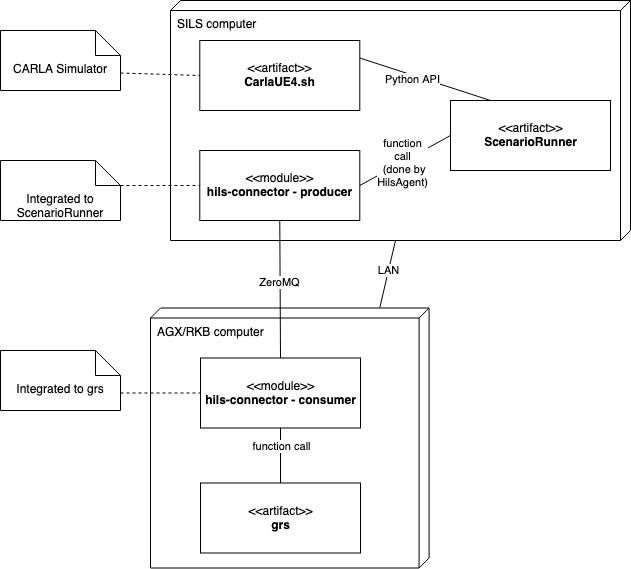
\includegraphics[width=0.4\textwidth]{resources/chapter-3/deployment-diagram-new-hils-EN.png}}
	\caption{HILS System Architecture}
	\label{section-3-hils-deployment-diagram}
\end{figure}

Then, as for how the system runs, it can be seen in
Fig.~\ref{section-3-hils-sequence-diagram}. Do note ScenarioRunner is called
``HILS agent'' in the diagram because HILS agent is the agent that is ran on
ScenarioRunner. To summarize how the system works:
\begin{enumerate}
	\item when CARLA steps, a sensor data is emitted,
	\item the producer component pushes it to the ZeroMQ socket,
	\item the consumer component waits for sensor data then pull from each
	      ZeroMQ socket,
	\item GRS will process that data to generate a control,
	\item the consumer component pushes the control to the ZeroMQ socket,
	\item the producer component will pull it and then send it to the
	      ScenarioRunner program, and
	\item ScenarioRunner will then apply the control to CARLA.
\end{enumerate}

\begin{figure}[htbp]
	\centerline{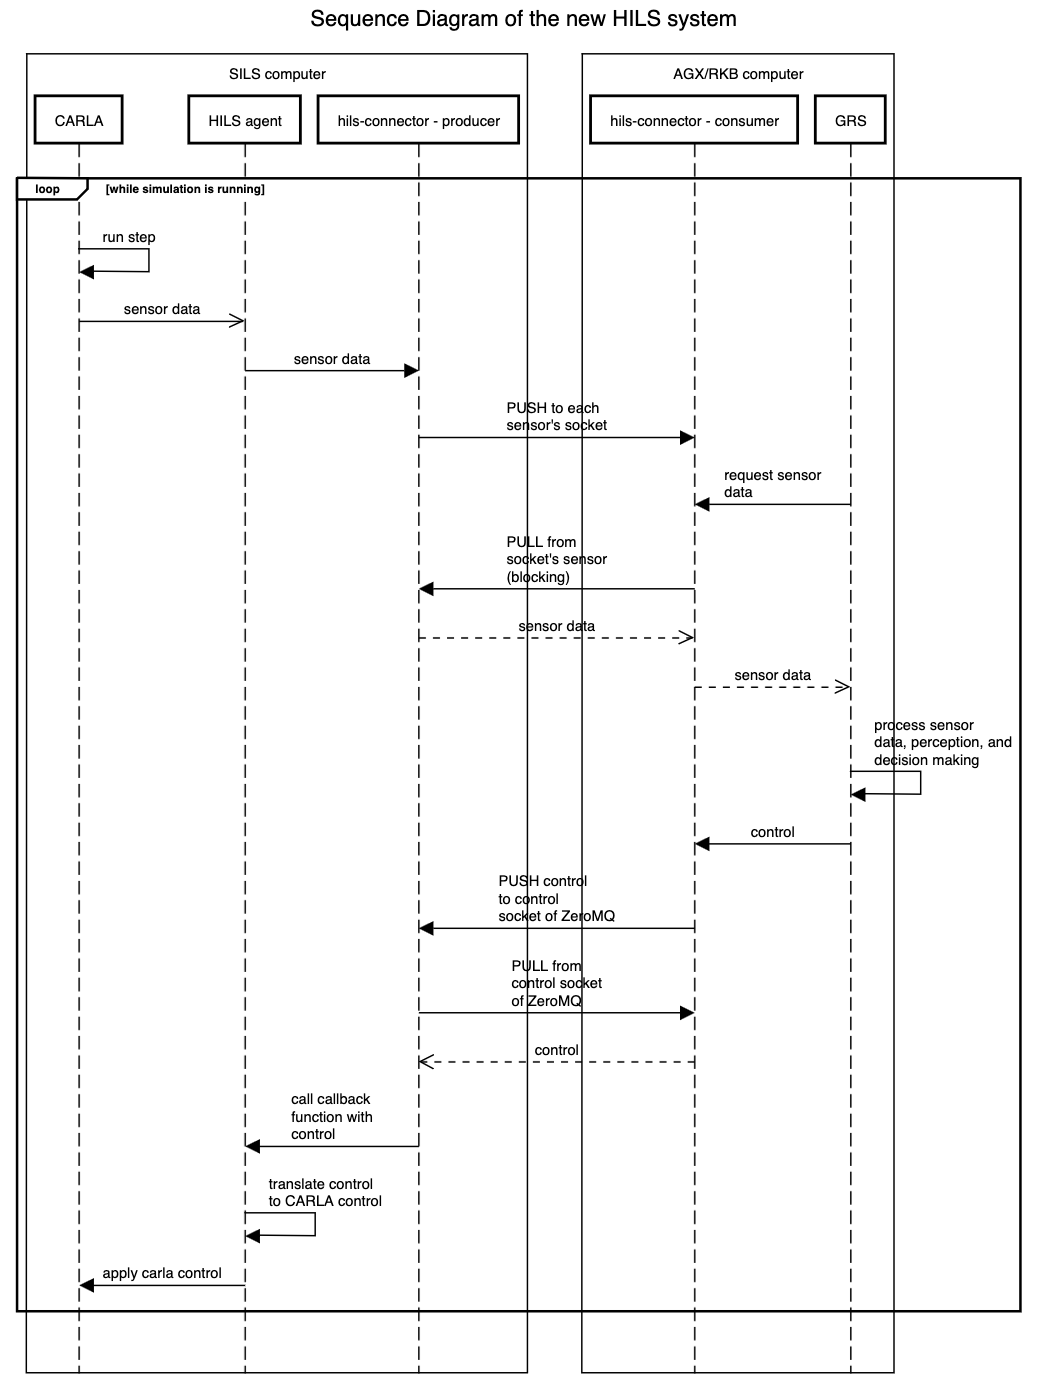
\includegraphics[width=0.5\textwidth]{resources/chapter-3/sequence-diagram-new-hils-kasar-EN.png}}
	\caption{HILS System Architecture}
	\label{section-3-hils-sequence-diagram}
\end{figure}

% \begin{table}[htbp]
% 	\caption{Table Type Styles}
% 	\label{tab1}
% 	\begin{center}
% 		\begin{tabular}{c c c c}
% 			\toprule
% 			\textbf{Table} & \multicolumn{3}{|c|}{\textbf{Table Column Head}}                                                         \\
% 			\cline{2-4}
% 			\textbf{Head}  & \textbf{\textit{Table column subhead}}           & \textbf{\textit{Subhead}} & \textbf{\textit{Subhead}} \\
% 			\midrule
% 			copy           & More table copy$^{\mathrm{a}}$                   &                           &                           \\
% 			\bottomrule
% 			\multicolumn{4}{l}{$^{\mathrm{a}}$Sample of a Table footnote.}
% 		\end{tabular}
% 	\end{center}
% \end{table}
\section{System Overview}

In this research, a library called ``hils-connector'' is created. The purpose of
this library is to connect the ScenarioRunner and GRS program. The
``hils-connector'' is the interface that allows both programs to exchange data.
The library itself has two components: ``consumer'' (consumes sensor data, used
by GRS) and ``producer'' (produces sensor data by forwarding sensor data from
CARLA to consumer, used by ScenarioRunner).

The approach to use a library is chosen to reduce coupling between the library
and both main programs. The library can be loaded and linked optionally during
runtime and compile time to make better use of both computers' resources.

The communication protocol/method that is chosen for is ZeroMQ. ZeroMQ is chosen
because of its minimalism which could lead to improvement in communication
latency. Previously, ROS 2 was also considered, but ROS 2 has a lot of
abstraction layers and isn't supported by the OS version in AGX/RKB computer.
ROS 2 uses DDS (data distribution service) for its transportation layer
\cite{doi:10.1126/scirobotics.abm6074_ros}, while ZeroMQ can directly use TCP or
any other transport protocol \cite{hurton_zmtp}.  The AGX/RKB computer runs
Ubuntu 18.04 which only supports up to ROS 1. Although a bridge between ROS 2
and ROS 1, that bridge would only add overhead in the communication process,
therefore ROS was not chosen.

Another communication protocol that was considered is HTTP, which is used in the
previous HILS system. HTTP is also not chosen because of the additional overhead
needed to parse header and status code which is not needed in the HILS system
\cite{rfc9110}. Thus, to maximize the usage of computer resource and reduce
possible overhead, ZeroMQ is chosen over HTTP.

With this library approach, the system architecture can be seen in
Fig.~\ref{section-4-hils-deployment-diagram}. The two main programs,
ScenarioRunner and GRS, are connected to each other using hils-connector in a
local area network. Each library components are then connected using ZeroMQ.
CARLA is connected to the ScenarioRunner program using the CARLA Python API's
function calls.

\begin{figure}[htbp]
	\centerline{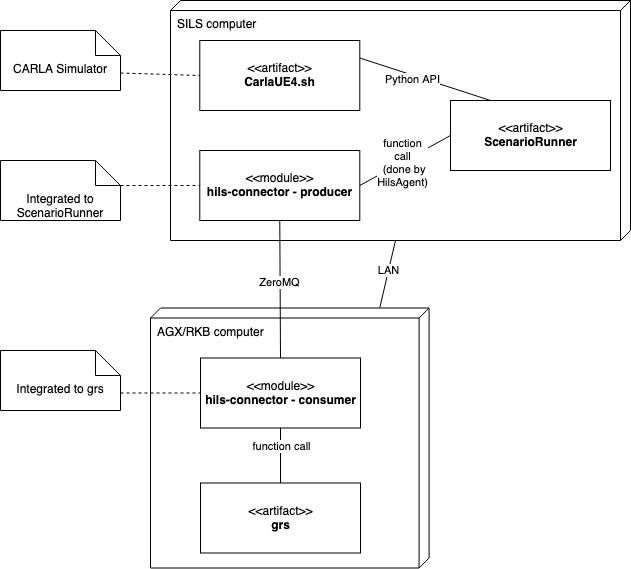
\includegraphics[width=0.4\textwidth]{resources/chapter-3/deployment-diagram-new-hils-EN.png}}
	\caption{HILS System Architecture}
	\label{section-4-hils-deployment-diagram}
\end{figure}

Then, as for how the system runs, it can be seen in
Fig.~\ref{section-4-hils-sequence-diagram}. Do note ScenarioRunner is called
``HILS agent'' in the diagram because HILS agent is the agent that is ran on
ScenarioRunner. To summarize how the system works:
\begin{enumerate}
	\item when CARLA steps, a sensor data is emitted,
	\item the producer component pushes it to the ZeroMQ socket,
	\item the consumer component waits for sensor data then pull from each
	      ZeroMQ socket,
	\item GRS will process that data to generate a control,
	\item the consumer component pushes the control to the ZeroMQ socket,
	\item the producer component will pull it and then send it to the
	      ScenarioRunner program, and
	\item ScenarioRunner will then apply the control to CARLA.
\end{enumerate}

\begin{figure}[htbp]
	\centerline{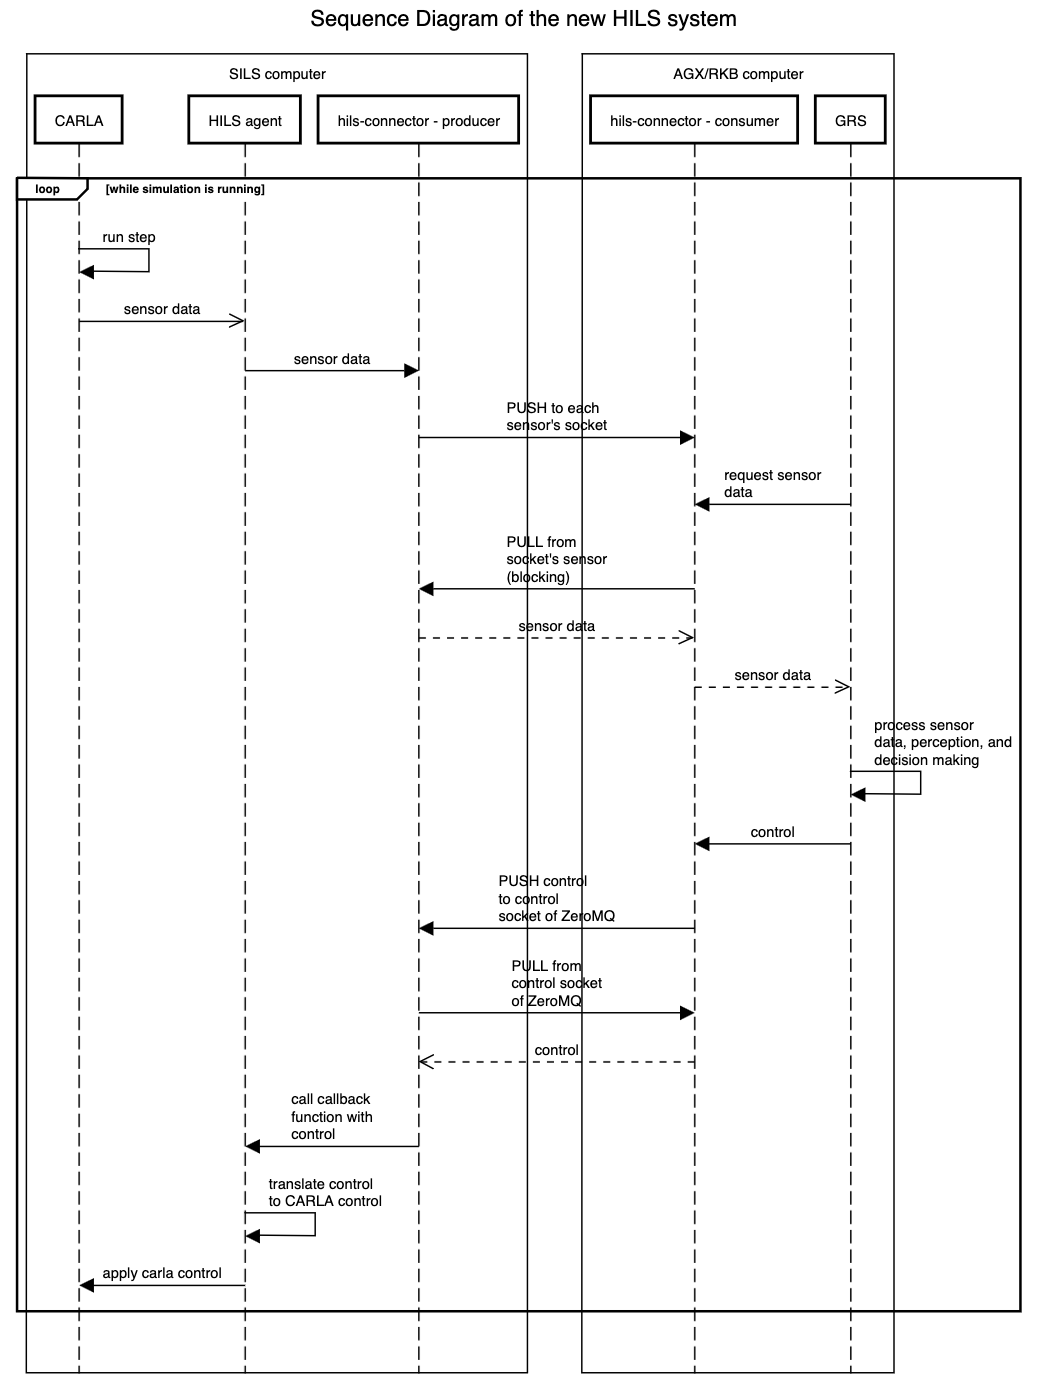
\includegraphics[width=0.5\textwidth]{resources/chapter-3/sequence-diagram-new-hils-kasar-EN.png}}
	\caption{HILS System Architecture}
	\label{section-4-hils-sequence-diagram}
\end{figure}

% \begin{table}[htbp]
% 	\caption{Table Type Styles}
% 	\label{tab1}
% 	\begin{center}
% 		\begin{tabular}{c c c c}
% 			\toprule
% 			\textbf{Table} & \multicolumn{3}{|c|}{\textbf{Table Column Head}}                                                         \\
% 			\cline{2-4}
% 			\textbf{Head}  & \textbf{\textit{Table column subhead}}           & \textbf{\textit{Subhead}} & \textbf{\textit{Subhead}} \\
% 			\midrule
% 			copy           & More table copy$^{\mathrm{a}}$                   &                           &                           \\
% 			\bottomrule
% 			\multicolumn{4}{l}{$^{\mathrm{a}}$Sample of a Table footnote.}
% 		\end{tabular}
% 	\end{center}
% \end{table}
\section{Testing and Results}

The testing will be done in two parts: implementation and performance testing.
The implementation testing tests the library implementation result, whether
sensor data can be used and a hardware-in-the-loop simulation can be done. The
performance testing tests, well, the HILS system performance.

\subsection{Testing Environment}

The implementation testing is done on AGX and SILS computers while performance
testing is done on RKB and SILS computer. The specification of RKB and SILS
computers can be seen in Table~\ref{tbl-section-5-computers-specs}. The RKB/AGX
and SILS computers are connected with a 1 Gbps link speed.

\begin{table}[htbp]
	\caption{SILS and RKB Computers Specification}
	\label{tbl-section-5-computers-specs}
	\begin{center}
		\begin{tabular}{r c c}
			\toprule
			                  & CPU & i9-10920X 12C/24T 3.50 GHz \\
			\textbf{SILS}     & RAM & 128 GB                     \\
			\textbf{computer} & GPU & 2x NVIDIA GeForce RTX 3090 \\
			                  & OS  & Ubuntu Linux 20.04         \\
			\midrule
			                  & CPU & i7-8700 6C/12T 3.20 GHz    \\
			\textbf{RKB}      & RAM & 16 GB                      \\
			\textbf{computer} & GPU & NVIDIA GeForce RTX 2070    \\
			                  & OS  & Ubuntu Linux 18.04         \\
			\bottomrule
		\end{tabular}
	\end{center}
\end{table}

\subsection{Implementation Testing}\label{section-4-implementation-testing}

The implementation testing tests the functionality of the library when used in a
running simulation. There are four criterias to be achieved in this category which are

\begin{enumerate}
	\item the speed shown in GRS is the same one from the virtual GNSS sensor,
	\item the camera feed shown in GRS is the same one from the virtual camera
	      sensor,
	\item the lidar images shown in GRS is the same one from the virtual lidar
	      sensor, and
	\item the tram in CARLA can move according to the control sent by GRS.
\end{enumerate}

The result of the implementation can be seen in
Fig.~\ref{fig-section-5-implementation-results}. It can be seen that the camera
feed shown in GRS (right monitor) is the same as the camera window in
ScenarioRunner which is taken from the virtual sensors directly (left monitor).

\begin{figure}[htbp]
	\centerline{\includegraphics[width=0.45\textwidth,trim={12cm 12cm 0 12cm},clip]{resources/chapter-4/HILS-system-running.png}}
	\caption{Implementation Result}
	\label{fig-section-5-implementation-results}
\end{figure}

\subsection{Performance Testing}

The performance testing is done on the RKB and SILS computer. The reason for
using RKB instead of AGX is, during the performance testing period, the AGX
computer was being used for field testing. There are two criterias for this
category:
\begin{enumerate}
	\item CARLA can maintain at least 2 FPS when simulation is running, and
	\item communication latency have to be faster compared to previous HILS
	      system.
\end{enumerate}
The requirement for CARLA to be running with at least 2 FPS comes from project
owner. Furthermore, there's a caveat to testing the second criteria, because the
previous HILS is not up to par in feature and too hard to start, the comparison
is done to a ``theoretical'' version of the previous HILS. The ``theoretical''
version of previous HILS is only implements some operations done in it instead
of the whole process. Moreover, the latency testing only uses GNSS and Camera
sensor. The lidar sensor isn't used because of technical difficulties during the
implementation.

In the performance test, latency is calculated by dividing round-trip time (RTT) by two.
It is calculated in ScenarioRunner/SILS computer side using camera sensor data
and using the formula in Eq.~\ref{eqn-section-5-rtt}.
\begin{equation}
	\label{eqn-section-5-rtt}
	\text{RTT} = T_{e} - T_{s} - t_p
\end{equation}
With:
\begin{table}[!h]
	\begin{tabular}{l l l}
		RTT     & : & round-trip time (in ms)                                  \\
		$T_{e}$ & : & timestamp control is received in ScenarioRunner (in ms)  \\
		$T_{s}$ & : & timestamp first camera segment is sent in ScenarioRunner \\
		        &   & (in ms)                                                  \\
		$t_p$   & : & processing time in GRS (in ms)
	\end{tabular}
\end{table}

$T_e$, $T_s$, and $t_p$ is taken before ZeroMQ library function is called. This
causes a small overhead in the RTT calculation.

The camera data is used to calculate RTT because it has a significantly large
size therefore, the camera data can show the worst case scenario.  Because the
size of the camera data, it can't be transmitted as a single packet using
ZeroMQ, instead it has to be sliced into a smaller segments. The RTT is
calculated from the first segment transmitted so the RTT is the time to send a
sensor data, not the time to send a single segment.

As for the latency calculation in ``theoretical'' previous HILS, it is started
from when the sensor data is sent and until the data is received on the other
side.

The performance testing's results can be seen in
Table~\ref{tbl-section-5-perf-result-statistics} and
Fig.~\ref{fig-section-5-carla-fps}. Using the new HILS implementation, CARLA can
run with 5--13 FPS. Addtionally, the average latency to send camera data is at
least 2.5x faster when compared to the previous HILS.

\begin{table}[!htbp]
	\caption{Performance Testing Statistics}
	\label{tbl-section-5-perf-result-statistics}
	\begin{center}
		\begin{tabular}{c c c}
			\toprule
			                       & Data count   & 1.000     \\
			\cline{2-3}
			                       & Average (ms) & 28,4245   \\
			\cline{2-3}
			                       & Std (ms)     & 4,68      \\
			\cline{2-3}
			\textbf{previous HILS} & Min (ms)     & 16        \\
			\cline{2-3}
			(``theoretical'')      & $Q_1$ (ms)   & 25        \\
			\cline{2-3}
			                       & $Q_2$ (ms)   & 28        \\
			\cline{2-3}
			                       & $Q_3$ (ms)   & 31        \\
			\cline{2-3}
			                       & Max (ms)     & 45,5      \\
			\midrule
			                       & Data count   & 16.891    \\
			\cline{2-3}
			                       & Average (ms) & 10,989965 \\
			\cline{2-3}
			                       & Std (ms)     & 2,248782  \\
			\cline{2-3}
			\textbf{new HILS}      & Min (ms)     & 4,5       \\
			\cline{2-3}
			                       & $Q_1$ (ms)   & 10        \\
			\cline{2-3}
			                       & $Q_2$ (ms)   & 11        \\
			\cline{2-3}
			                       & $Q_3$ (ms)   & 12,5      \\
			\cline{2-3}
			                       & Max (ms)     & 19,5      \\
			\bottomrule
		\end{tabular}
	\end{center}
\end{table}

\begin{figure}[htbp]
	\centerline{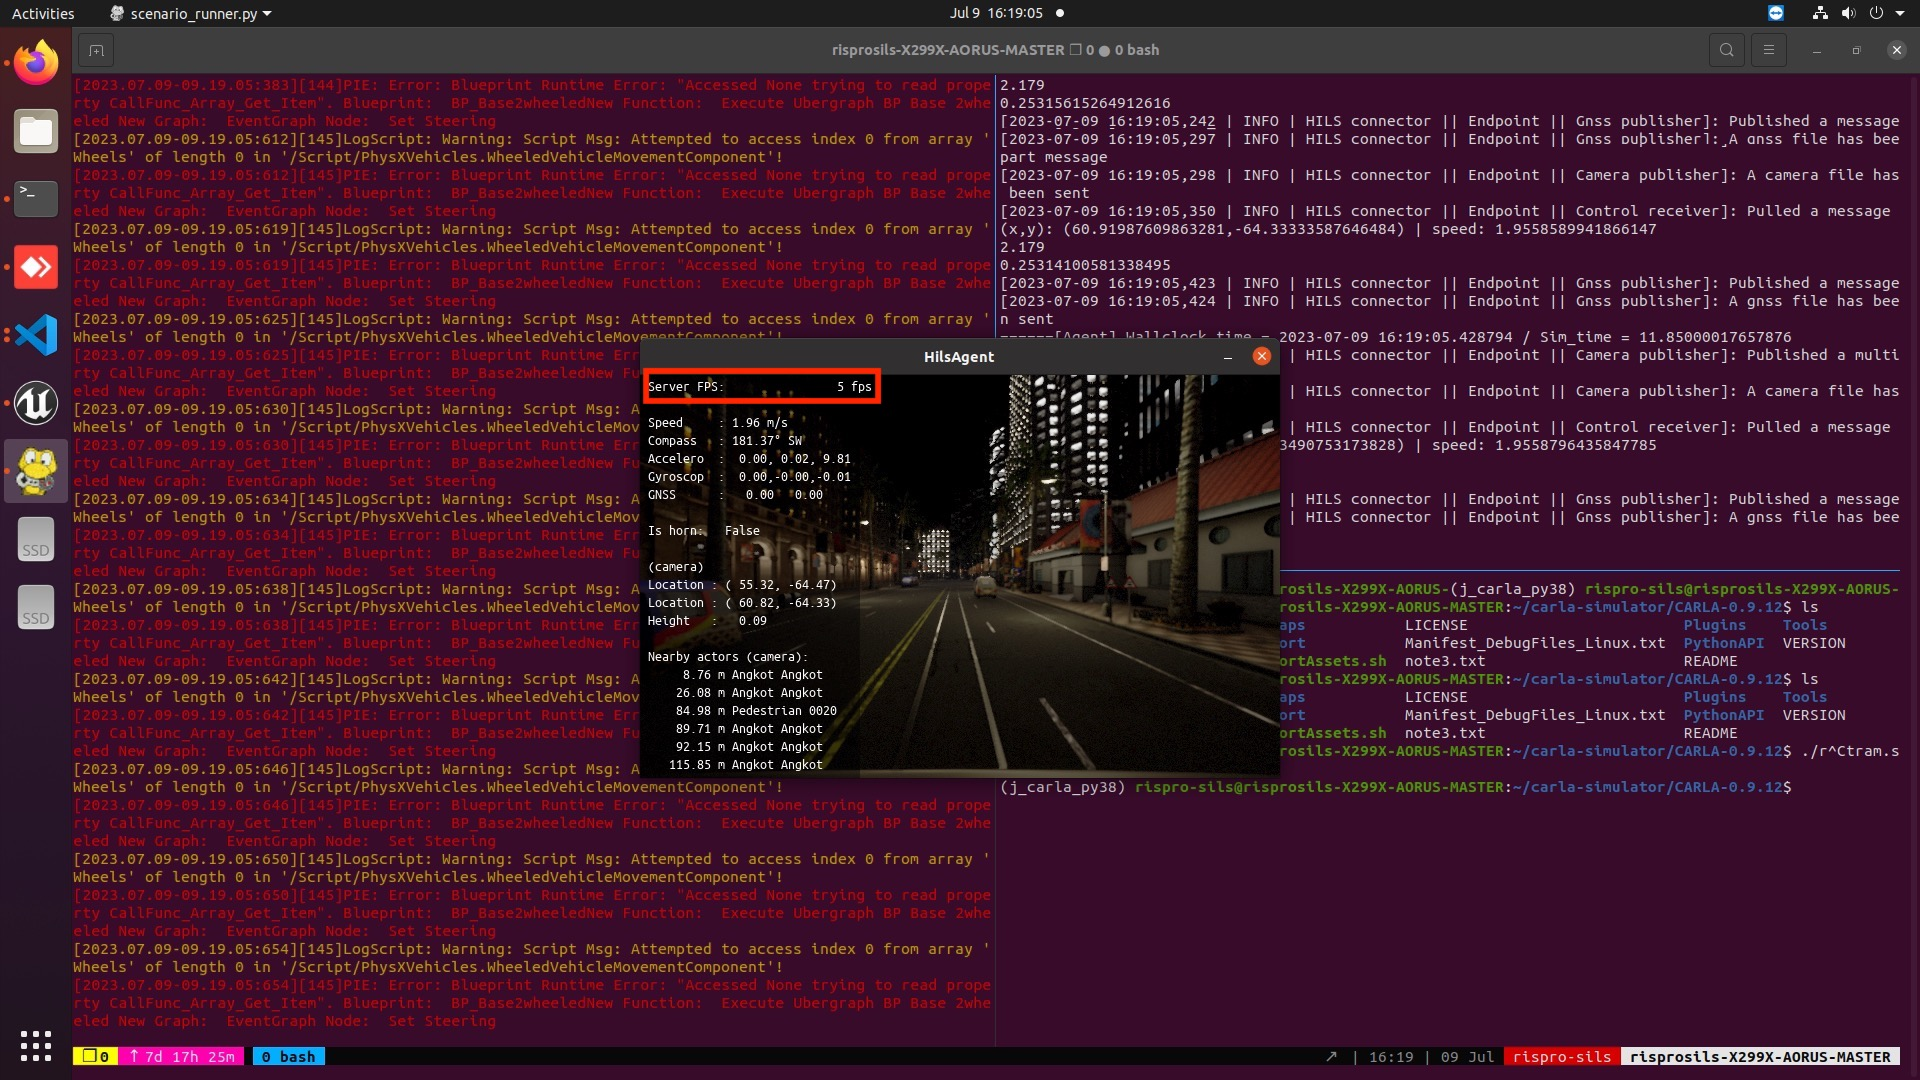
\includegraphics[width=0.45\textwidth,trim={22.5cm 10.5cm 22.5cm 12cm},clip]{resources/chapter-4/CARLA-5FPS.JPG}}
	\centerline{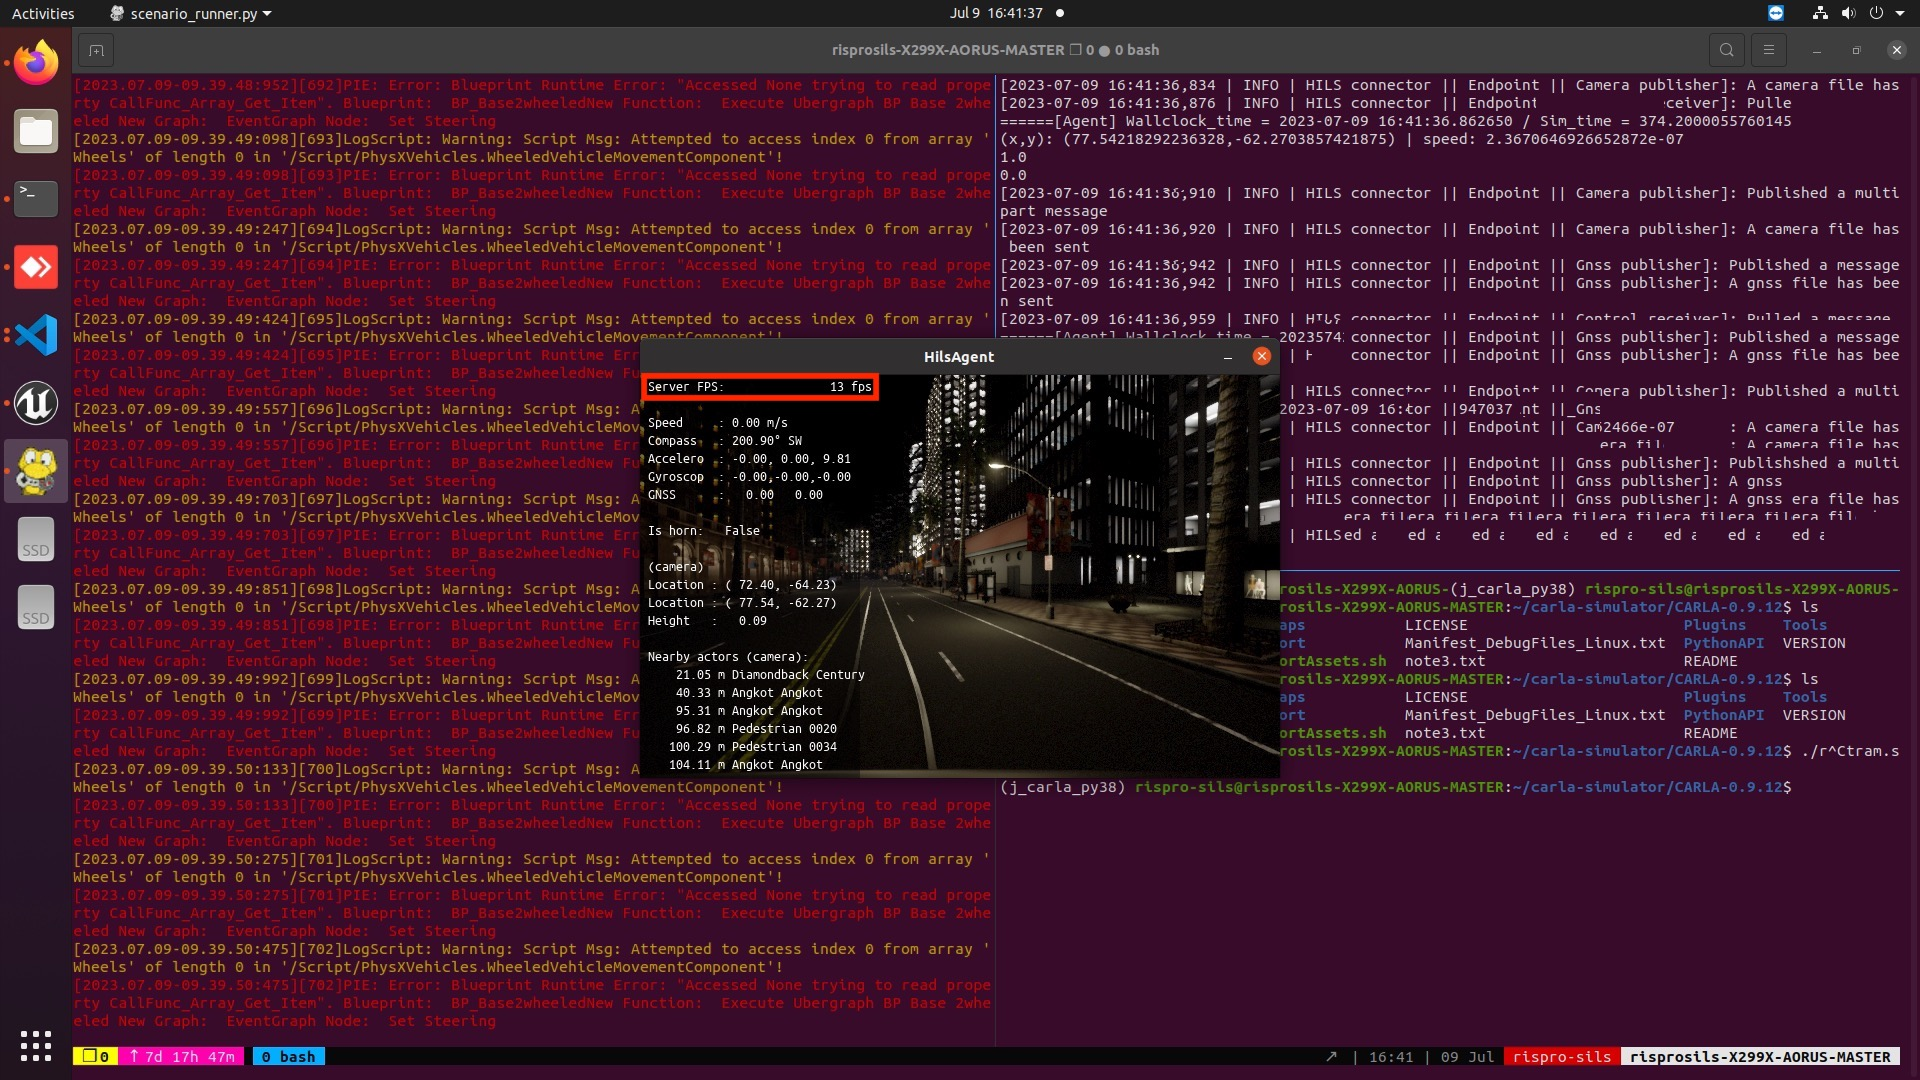
\includegraphics[width=0.45\textwidth,trim={22.5cm 10.5cm 22.5cm 12cm},clip]{resources/chapter-4/CARLA-13FPS.JPG}}
	\caption{CARLA FPS}
	\label{fig-section-5-carla-fps}
\end{figure}
\section{Testing and Results}

The testing is done in two parts: implementation and performance testing.  The
implementation testing tests the library implementation result, whether sensor
data can be used and a hardware-in-the-loop simulation can be done. The
performance testing tests, well, the HILS system performance.

\subsection{Testing Environment}

The implementation testing is done on AGX and SILS computers while performance
testing is done on RKB and SILS computer. The specification of RKB and SILS
computers can be seen in Table~\ref{tbl-section-6-computers-specs}. The RKB/AGX
and SILS computers are connected with a 1 Gbps link speed.

\begin{table}[htbp]
	\caption{SILS and RKB Computers Specification}
	\label{tbl-section-6-computers-specs}
	\begin{center}
		\begin{tabular}{r c c}
			\toprule
			                  & CPU & i9-10920X 12C/24T 3.50 GHz \\
			\textbf{SILS}     & RAM & 128 GB                     \\
			\textbf{computer} & GPU & 2x NVIDIA GeForce RTX 3090 \\
			                  & OS  & Ubuntu Linux 20.04         \\
			\midrule
			                  & CPU & i7-8700 6C/12T 3.20 GHz    \\
			\textbf{RKB}      & RAM & 16 GB                      \\
			\textbf{computer} & GPU & NVIDIA GeForce RTX 2070    \\
			                  & OS  & Ubuntu Linux 18.04         \\
			\bottomrule
		\end{tabular}
	\end{center}
\end{table}

\subsection{Implementation Testing}\label{section-4-implementation-testing}

The implementation testing tests the functionality of the library when used in a
running simulation. There are four criteria to be achieved in this category
which are
\begin{enumerate}
	\item the speed shown in GRS is the same one from the virtual GNSS sensor,
	\item the camera feed shown in GRS is the same one from the virtual camera
	      sensor,
	\item the lidar images shown in GRS is the same one from the virtual lidar
	      sensor, and
	\item the tram in CARLA can move according to the control sent by GRS.
\end{enumerate}

The result of the implementation can be seen in
Fig.~\ref{fig-section-6-implementation-results}. It can be seen that the camera
feed shown in GRS (right monitor) is the same as the camera window in
ScenarioRunner which is taken from the virtual sensors directly (left monitor).

\begin{figure}[htbp]
	\centerline{\includegraphics[width=0.45\textwidth,trim={12cm 12cm 0 12cm},clip]{resources/chapter-4/HILS-system-running.png}}
	\caption{Implementation Result}
	\label{fig-section-6-implementation-results}
\end{figure}

\subsection{Performance Testing}

The performance testing is done on the RKB and SILS computers. The reason for
using RKB instead of AGX is, during the performance testing period, the AGX
computer was being used for field testing. There are two criteria for this
category:
\begin{enumerate}
	\item CARLA can maintain at least 2 FPS when a simulation is running, and
	\item communication latency has to be faster compared to the previous HILS
	      system.
\end{enumerate}
The requirement for CARLA to be running with at least 2 FPS comes from the
autonomous tram project owner. Furthermore, there's a caveat to testing the
second criterion, because the previous HILS is not up to par in features and too
hard to start, the comparison is done to a ``theoretical'' version of the
previous HILS. The ``theoretical'' version of the previous HILS only implements
some operations done in it instead of the whole process. Moreover, the latency
testing only uses a GNSS and a camera sensor. The lidar sensor isn't used
because of technical difficulties during the implementation.

In the performance test, latency is calculated by dividing round-trip time (RTT) by two.
It is calculated in ScenarioRunner/SILS computer side using camera sensor data
and using the formula in Eq.~\ref{eqn-section-6-rtt}.
\begin{equation}
	\label{eqn-section-6-rtt}
	\text{RTT} = T_{e} - T_{s} - t_p
\end{equation}
With:
\begin{table}[!h]
	\begin{tabular}{l l l}
		RTT     & : & round-trip time (in ms)                                  \\
		$T_{e}$ & : & timestamp control is received in ScenarioRunner (in ms)  \\
		$T_{s}$ & : & timestamp first camera segment is sent in ScenarioRunner \\
		        &   & (in ms)                                                  \\
		$t_p$   & : & processing time in GRS (in ms)
	\end{tabular}
\end{table}

$T_e$, $T_s$, and $t_p$ are taken before the ZeroMQ library function is called.
This causes a small overhead in the RTT calculation.

The camera data is used to calculate RTT because it has a significantly large
size therefore, the camera data can show the worst-case scenario. Because of the
size of the camera data, it can't be transmitted as a single packet using
ZeroMQ, instead, it has to be sliced into smaller segments. The RTT is
calculated from the first segment transmitted so the RTT is the time to send
sensor data, not the time to send a single segment.

As for the latency calculation in the ``theoretical'' previous HILS, it is
started from when the sensor data is sent and until the data is received on the
other side.

The performance testing results can be seen in
Table~\ref{tbl-section-6-perf-result-statistics} and
Fig.~\ref{fig-section-6-carla-fps}. Using the new HILS implementation, CARLA can
run with 5--13 FPS. Additionally, the average latency to send camera data is
10.99 ms which is at least 2.5x faster when compared to the previous HILS.

\begin{table}[!htbp]
	\caption{Performance Testing Statistics}
	\label{tbl-section-6-perf-result-statistics}
	\begin{center}
		\begin{tabular}{c c c}
			\toprule
			                       & Data count   & 1.000     \\
			\cline{2-3}
			                       & Average (ms) & 28,4245   \\
			\cline{2-3}
			                       & Std (ms)     & 4,68      \\
			\cline{2-3}
			\textbf{previous HILS} & Min (ms)     & 16        \\
			\cline{2-3}
			(``theoretical'')      & $Q_1$ (ms)   & 25        \\
			\cline{2-3}
			                       & $Q_2$ (ms)   & 28        \\
			\cline{2-3}
			                       & $Q_3$ (ms)   & 31        \\
			\cline{2-3}
			                       & Max (ms)     & 45,5      \\
			\midrule
			                       & Data count   & 16.891    \\
			\cline{2-3}
			                       & Average (ms) & 10,989965 \\
			\cline{2-3}
			                       & Std (ms)     & 2,248782  \\
			\cline{2-3}
			\textbf{new HILS}      & Min (ms)     & 4,5       \\
			\cline{2-3}
			                       & $Q_1$ (ms)   & 10        \\
			\cline{2-3}
			                       & $Q_2$ (ms)   & 11        \\
			\cline{2-3}
			                       & $Q_3$ (ms)   & 12,5      \\
			\cline{2-3}
			                       & Max (ms)     & 19,5      \\
			\bottomrule
		\end{tabular}
	\end{center}
\end{table}

\begin{figure}[htbp]
	\centerline{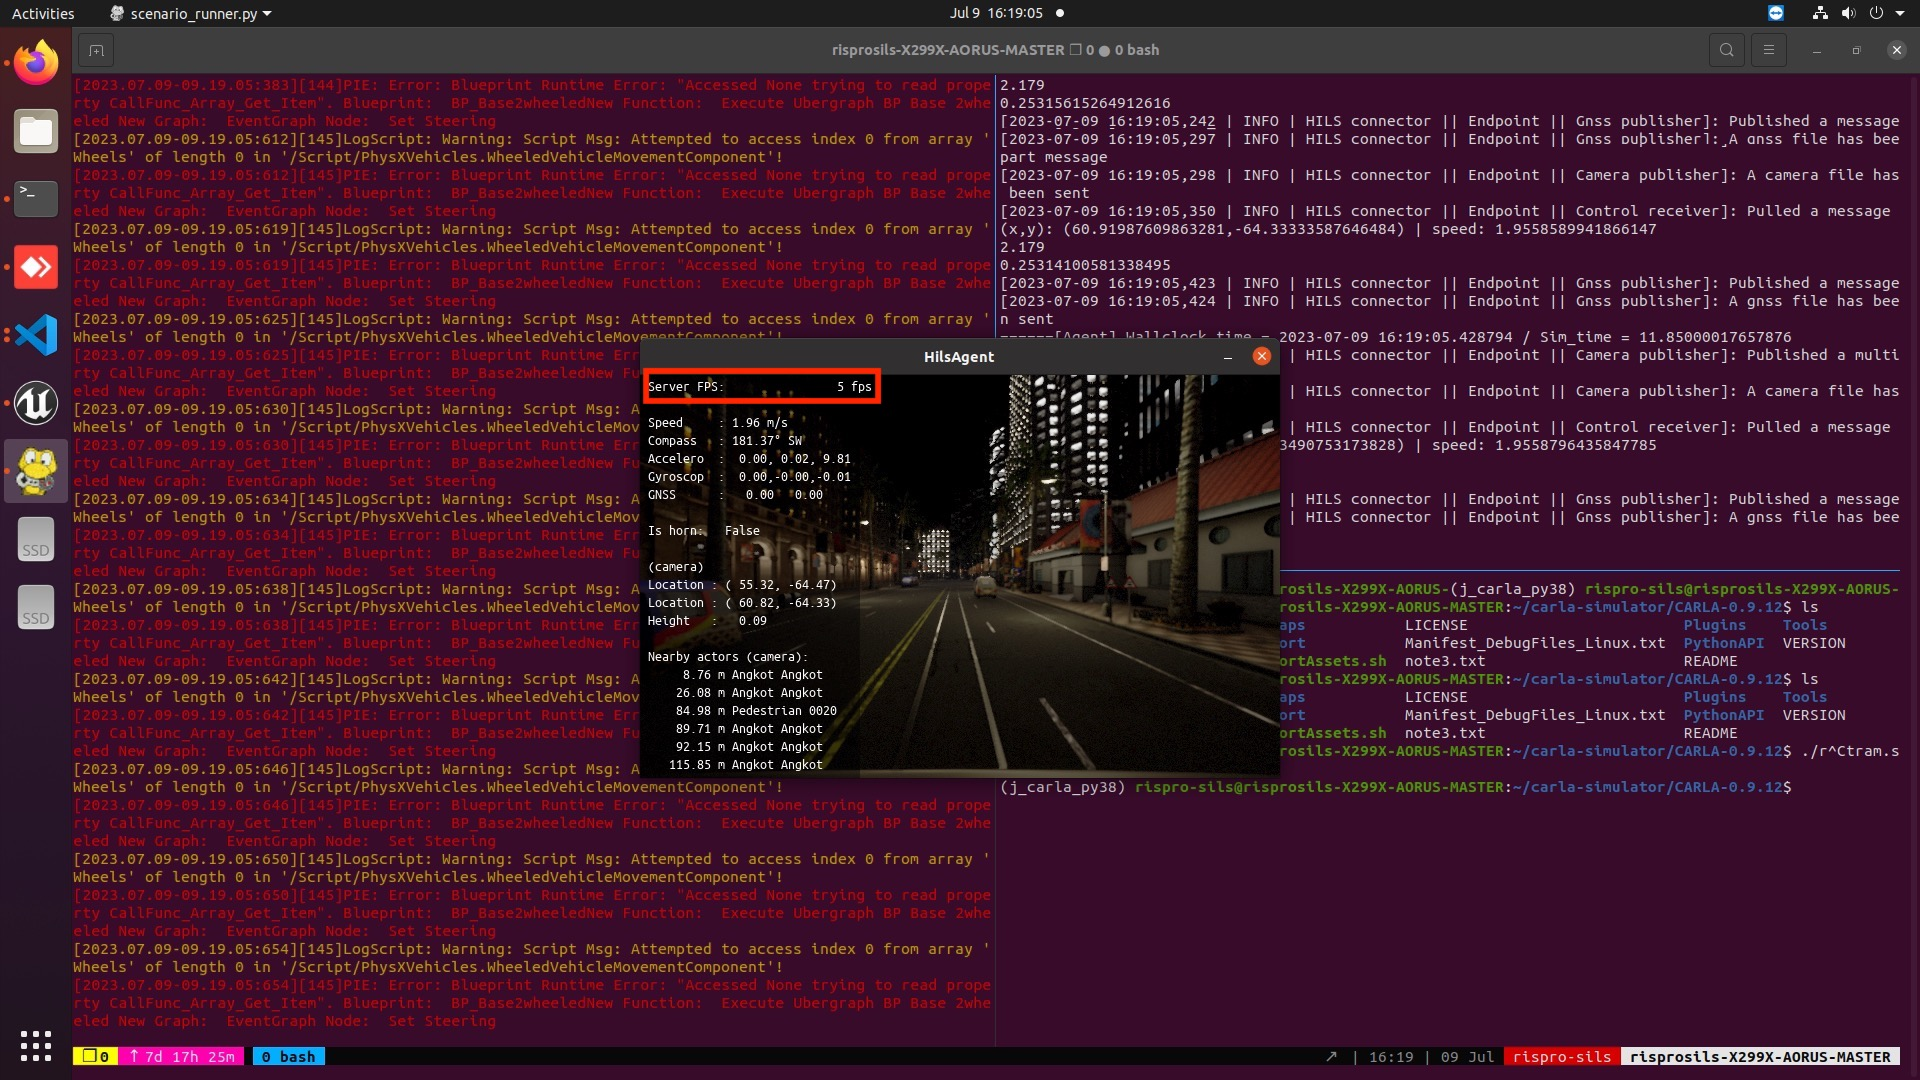
\includegraphics[width=0.45\textwidth,trim={22.5cm 10.5cm 22.5cm 12cm},clip]{resources/chapter-4/CARLA-5FPS.JPG}}
	\centerline{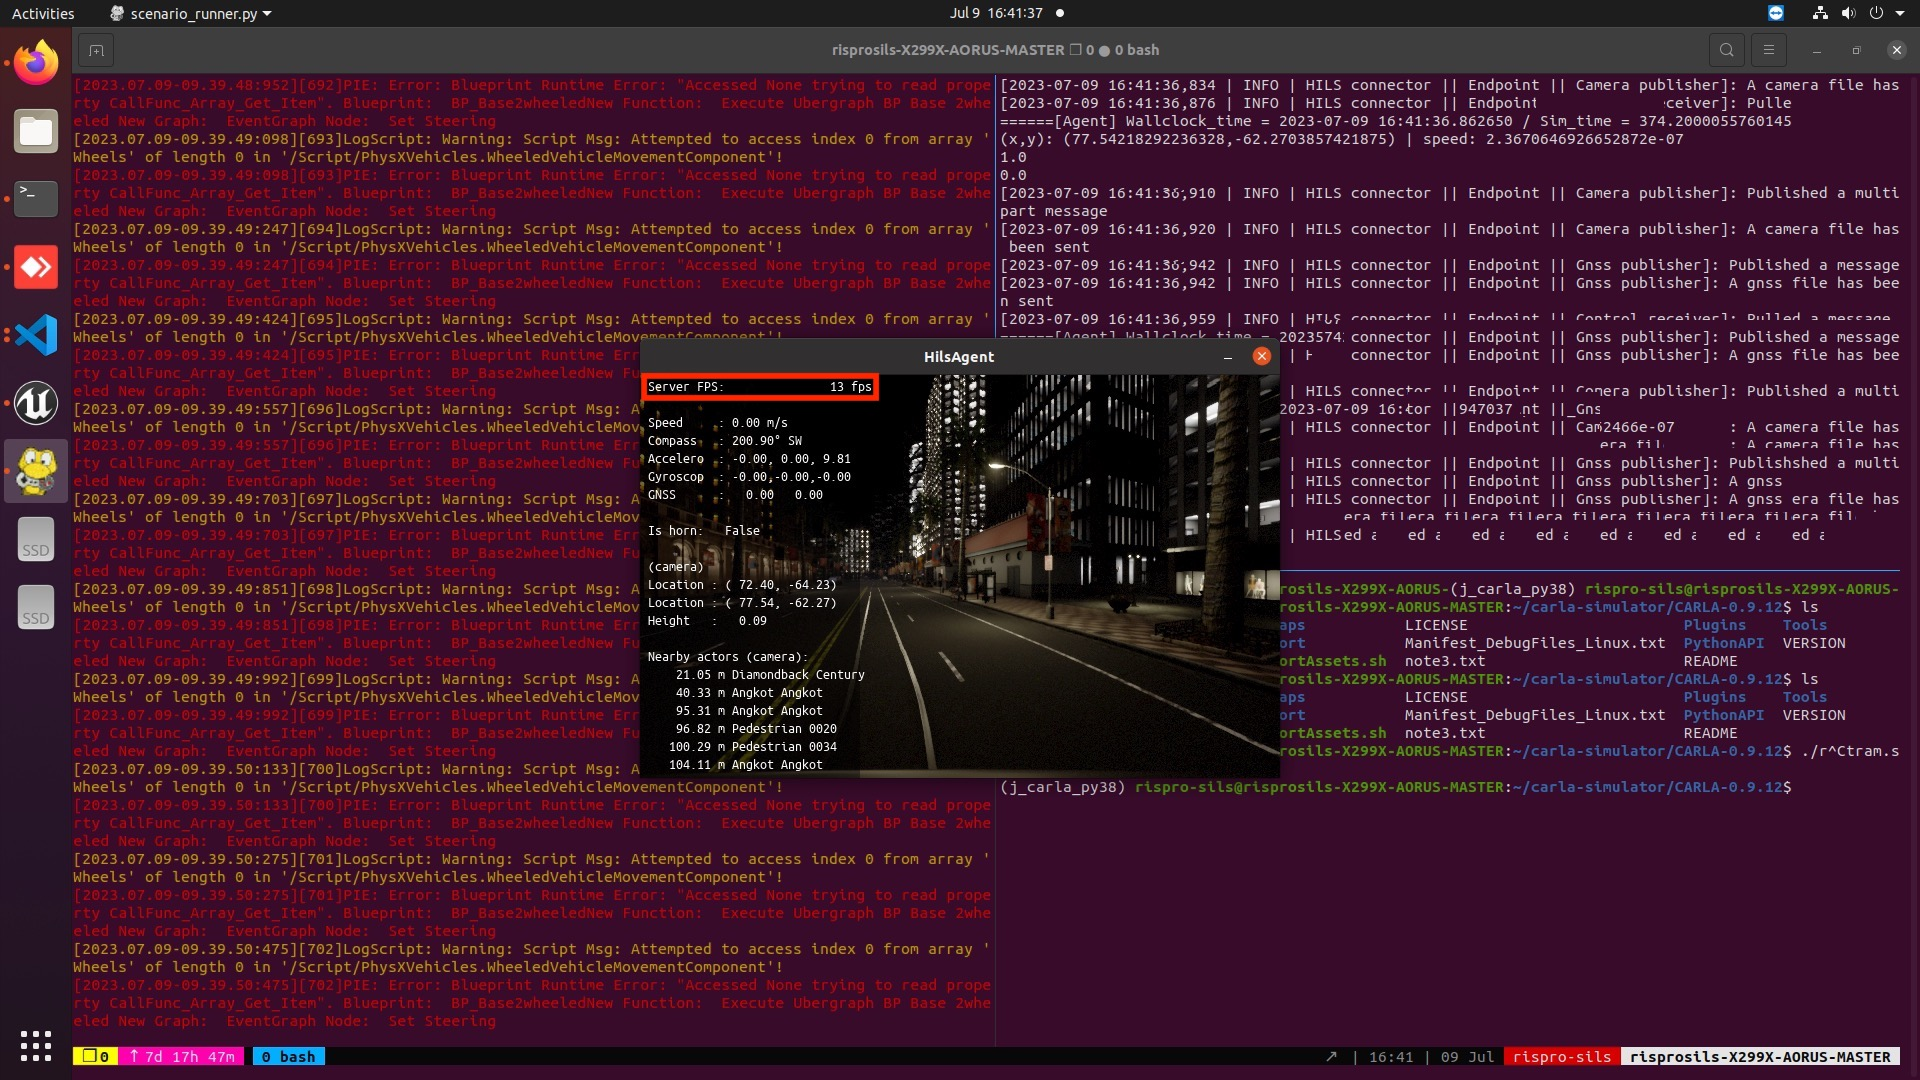
\includegraphics[width=0.45\textwidth,trim={22.5cm 10.5cm 22.5cm 12cm},clip]{resources/chapter-4/CARLA-13FPS.JPG}}
	\caption{CARLA FPS}
	\label{fig-section-6-carla-fps}
\end{figure}
\section{Results Analysis and Discussion}

\subsection{Implementation Testing}

The implementation testing is successful as can be seen in
Section~\ref{section-4-implementation-testing}. This means the new HILS system
can use virtual sensor data for simulation.

\subsection{Performance Testing}

The performance improvement is achieved by eliminating unneeded I/O operations.
The previous HILS implementation needs 8 I/O operations just to send a single
data (the ``theoretical'' version only implements 4). The computers' resource
usage is not yet saturated when the testing is done, which further shows that
the improvement gained comes software adjustments.

Although it has to be noted that there is a technical difficulty in implementing
lidar sensors. Even though the lidar sensor is already usable, as proven in
implementation testing, it inhibits the performance of the simulation. Lidar
sensor slows down the performance because to get the whole lidar image CARLA
needs to run a few simulation steps first, unlike camera and GNSS where only one
step is needed. CARLA needs to run a few simulation steps because to get the
whole lidar image the lidar has to do a full rotation. Each simulation step
only rotates the lidar by some degree, therefore a few simulation steps are
needed to achieve the full lidar rotation.

\section*{Acknowledgment}

The preferred spelling of the word ``acknowledgment'' in America is without
an ``e'' after the ``g''. Avoid the stilted expression ``one of us (R. B.
G.) thanks $\ldots$''. Instead, try ``R. B. G. thanks$\ldots$''. Put sponsor

\printbibliography

\vspace{12pt}
\color{red}
IEEE conference templates contain guidance text for composing and formatting conference papers. Please ensure that all template text is removed from your conference paper prior to submission to the conference. Failure to remove the template text from your paper may result in your paper not being published.

\end{document}